
\chapter{Kvantové počítače}\label{ch:quantum_computers}

Kvantové počítače predstavujú zásadný posun v chápaní a realizácii výpočtových procesov. Na rozdiel od klasických počítačov, ktoré pracujú s bitmi nadobúdajúcimi hodnotu 0 alebo 1, kvantové počítače využívajú kvantové bity — \textit{qubity} — ktoré môžu existovať v stave superpozície a sú schopné vytvárať prepletenie (\textit{entanglement}). To im umožňuje paralelné spracovanie informácií a vykonávanie výpočtov, ktoré sú pre klasické zariadenia výpočtovo neúnosné \cite{Gill2020_QuantumComputingTaxonomy}.

\section{Typy kvantových počítačov}\label{sec:typy-kvantovych-pocitacov}

Existuje viacero typov kvantových počítačov, ktoré sa líšia implementáciou qubitov, použitými fyzikálnymi princípmi aj spôsobom interakcie medzi nimi. Medzi najvýznamnejšie patria:

\begin{itemize}
  \item \textbf{Supravodivé kvantové počítače}~\cite{AdvancementsSQC2025} – podľa dostupných zdrojov sú založené na supravodivých elektrických obvodoch prevádzkovaných pri extrémne nízkych teplotách. Takéto podmienky umožňujú vznik kvantových stavov v makroskopických systémoch. Qubity sú realizované v transmonovej architektúre, pričom manipulácia so stavmi sa vykonáva prostredníctvom riadených mikrovlnných impulzov. Tento prístup využívajú veľkí technologickí poskytovatelia ako IBM, Google, Rigetti alebo IQM.

  \item \textbf{Kvantové počítače založené na zachytených iónoch (\textit{trapped ions})}~\cite{Wineland1998_trapped_ion_primer} – literatúra opisuje tieto systémy ako sústavu jednotlivých iónov uväznených elektromagnetickým poľom. Kvantová informácia sa ukladá do energetických stavov iónov a operácie sa vykonávajú pomocou presne riadených laserových impulzov. Technológiu aktívne rozvíjajú spoločnosti IonQ a Honeywell.

  \item \textbf{Fotónové kvantové počítače}~\cite{Slussarenko2019_photonic_review} – vychádzajú z využitia fotónov ako nositeľov kvantovej informácie. Podľa odborných zdrojov sú obzvlášť vhodné pre aplikácie v kvantovej komunikácii a distribuovaných systémoch, keďže fotóny je možné efektívne prenášať na veľké vzdialenosti.

  \item \textbf{Topologické kvantové počítače}~\cite{Nayak2007_nonabelian_anyons} – predstavujú prístup, ktorý je podľa literatúry stále vo fáze experimentálneho výskumu. Ich hlavná idea spočíva v použití topologických kvantových stavov, ktoré by mali poskytovať vyššiu odolnosť voči chybám a zjednodušovať korekciu kvantových chýb.
\end{itemize}

Každý z týchto prístupov má svoje výhody aj nevýhody – supravodivé systémy sú rýchle, no citlivé na dekoherenciu; iónové počítače sú stabilnejšie, ale pomalšie a náročnejšie na škálovanie. Pre účely tejto práce bol zvolený supravodivý systém \textbf{IQM Emerald}~\cite{IQMEmerald}, ktorý je dostupný prostredníctvom platformy \textit{Amazon Braket}.

\section{Kvantové tunelovanie}\label{sec:kvantove-tunelovanie}

Kvantové tunelovanie je jav, pri ktorom častica prechádza energetickou bariérou, ktorú by podľa klasickej fyziky prekonať nemohla. Tento efekt je dôsledkom vlnovej povahy častíc a neurčitosti ich polohy a energie. V kontexte kvantových počítačov sa tunelovanie využíva najmä v supravodivých systémoch, kde elektróny môžu prechádzať cez tenkú izolačnú vrstvu (Josephsonov prechod), čo umožňuje vznik kvantového správania makroskopického elektrického prúdu. Tento princíp je základom pre tvorbu \textit{transmon} qubitov používaných v systéme IQM Emerald.

\clearpage

\section{Použitý systém: IQM Emerald}\label{sec:pouzity-system-iqm-emerald}

Kvantový počítač \textbf{IQM Emerald} využíva procesor \textit{IQM Crystal} s 54 qubitmi, založený na technológii supravodivých \textit{transmonových qubitov}. Tieto qubity sú usporiadané do štvorcovej mriežky a navzájom prepojené prostredníctvom nastaviteľných väzieb (\textit{tunable couplers}), ktoré umožňujú vysokú úroveň konektivity medzi jednotlivými prvkami systému ako je zobrazené na obrázku~\ref{fig:iqm_layout}. Architektúra zariadenia podporuje ľubovoľné rotácie okolo osí X a Y ako natívne jednobitové kvantové operácie a využíva bránu \textit{CZ} (\textit{controlled-Z}) ako svoju natívnu dvojbitovú operáciu.

Tieto vlastnosti robia z počítača IQM Emerald univerzálnu platformu pre kvantové výpočty založené na supravodivých obvodoch, ktorá je vhodná na experimentálne aj aplikačné použitie. Informácie o architektúre a parametroch zariadenia boli čerpané z oficiálneho zdroja výrobcu~\cite{IQMEmerald}.

\begin{figure}[H]
  \centering
  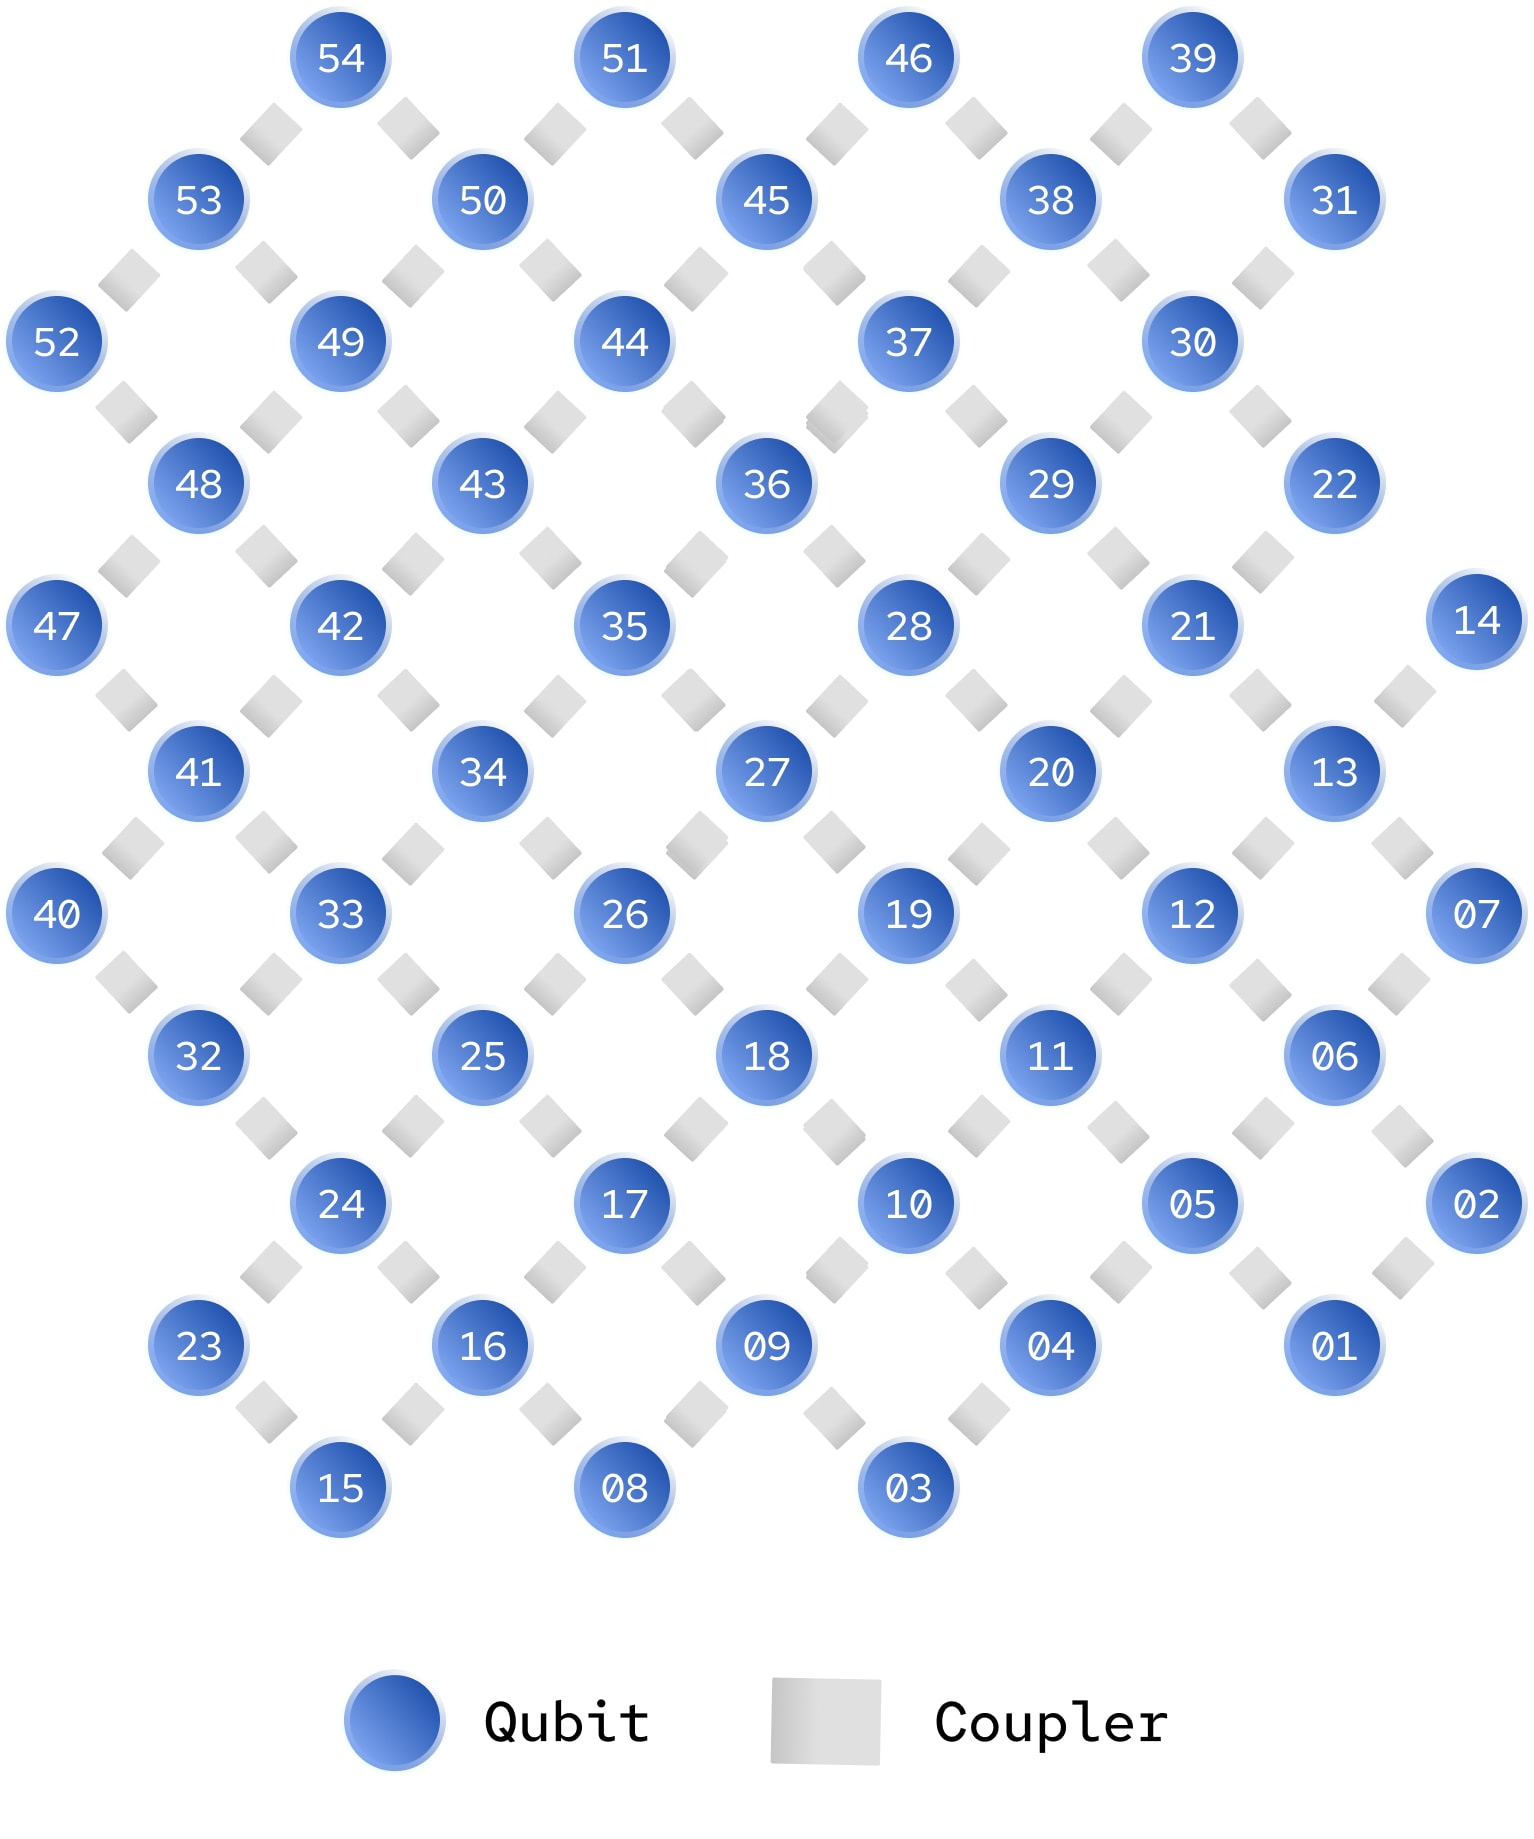
\includegraphics[width=0.65\textwidth]{images/IQMEmerald}
  \caption{Rozloženie qubitov a prepojovacích článkov (\textit{couplers}) v kvantovom procesore IQM Crystal, ktorý je súčasťou systému IQM Emerald. Každý modrý bod reprezentuje jeden supravodivý transmonový qubit a sivé štvorce znázorňujú nastaviteľné väzby medzi nimi.}
  \label{fig:iqm_layout}
\end{figure}

\section{Qubit}\label{sec:qubit}

Qubit (\textit{quantum bit}), ako bol definovaný v publikácii~\cite{hughes2021qubit}, je základná jednotka kvantovej informácie. Na rozdiel od klasického bitu, ktorý môže nadobúdať hodnotu 0 alebo 1, qubit môže existovať v superpozícii týchto stavov, teda v akejkoľvek kombinácii stavov $\lvert 0 \rangle$ a $\lvert 1 \rangle$:

\begin{equation}
  \lvert \psi \rangle = \alpha \lvert 0 \rangle + \beta \lvert 1 \rangle,
  \label{eq:qubit_state}
\end{equation}


kde $\alpha$ a $\beta$ sú komplexné koeficienty, pričom platí $\lvert \alpha \rvert^2 + \lvert \beta \rvert^2 = 1$. Stav qubitu sa mení pomocou kvantových brán — matematických operácií, ktoré zodpovedajú fyzikálnym manipuláciám so systémom (napr. rotáciám, pulzom či interakciám medzi qubitmi), ako je zobrazené na obrázku~\ref{fig:qbit_sphere}.

\begin{figure}[htbp]
  \centering
  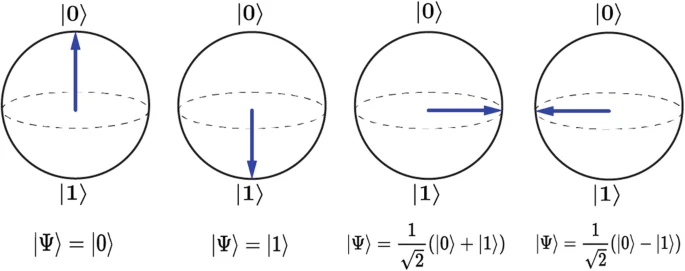
\includegraphics[width=0.8\textwidth]{images/QubitSfere}
  \caption{Stav qubitov znázornený pomocou šípu na Blochovej sfére.}
  \label{fig:qbit_sphere}
\end{figure}

\section{Kvantové logické brány}\label{sec:kvantove-logicke-brany}

Kvantové brány sú operácie, ktoré menia stav qubitov. Medzi základné patria:
\begin{itemize}
  \item \textbf{Hadamardova brána (H)}~\cite{nielsen_chuang_2010} – vytvára superpozíciu stavov $\lvert 0 \rangle$ a $\lvert 1 \rangle$:
  \begin{equation}
    H\lvert 0 \rangle = \frac{1}{\sqrt{2}}(\lvert 0 \rangle + \lvert 1 \rangle), \quad H\lvert 1 \rangle = \frac{1}{\sqrt{2}}(\lvert 0 \rangle - \lvert 1 \rangle).,
    \label{eq:hadamar_gate}
  \end{equation}

  \item \textbf{CNOT brána (Controlled-NOT)}~\cite{nielsen_chuang_2010} – dvojqubitová operácia, ktorá invertuje cieľový qubit iba vtedy, ak je riadiaci qubit v stave $\lvert 1 \rangle$. Predstavuje základnú logickú bránu pre tvorbu kvantových prepletených stavov.
\end{itemize}

\section{Tvorba Bellových párov}\label{sec:tvorba-bellovych-parov}

Bellove páry predstavujú základný koncept kvantovej teórie informácie a jeden z najvýznamnejších prejavov kvantového prepletenia. Ide o špeciálny typ dvojsystémových kvantových stavov, v ktorých stav jedného qubitu nemožno popísať nezávisle od stavu druhého, bez ohľadu na vzdialenosť medzi nimi. Tento jav predstavuje priamy rozpor s klasickými predstavami o lokálnosti a determinizme, ktoré boli základom fyziky až do polovice 20. storočia.

Matematicky sa Bellove páry vytvárajú aplikáciou Hadamardovej brány a následne CNOT brány na počiatočný stav $\lvert 00 \rangle$. Týmto postupom sa vytvorí kvantová superpozícia, v ktorej oba qubity nadobúdajú prepletený stav:

\begin{equation}
  \lvert \Phi^+ \rangle = \frac{1}{\sqrt{2}}(\lvert 00 \rangle + \lvert 11 \rangle),
  \label{eq:bell_pair_qubit_state}
\end{equation}

čo je jeden zo štyroch tzv. Bellových stavov. Tieto stavy sú charakteristické svojou dokonalou kvantovou koreláciou, ktorá nemá žiadny klasický ekvivalent. Ak dôjde k meraniu jedného qubitu, výsledok druhého je okamžite určený, bez ohľadu na vzdialenosť medzi nimi. Tento jav bol po prvýkrát teoreticky sformulovaný fyzikom Johnom Stewartom Bellom v prelomovej práci \textit{On the Einstein Podolsky Rosen Paradox}~\cite{PhysicsPhysiqueFizika.1.195}, ktorá položila základy celej modernej kvantovej teórie informácie.

Bellov príspevok spočíval v odvodení tzv. \textit{Bellových nerovností}, ktoré predstavujú matematické kritérium na rozlíšenie medzi kvantovými a klasickými (lokálnymi) koreláciami. Experimentálne porušenie týchto nerovností v nasledujúcich desaťročiach, v moderných „loophole-free“ testoch~\cite{shalm2015strong}, jednoznačne potvrdilo, že kvantová mechanika opisuje svet pravdepodobnostne a že prepletenie je reálny, fyzikálne merateľný jav.

Tento princíp tvorí základ celej tejto práce. Na ňom je postavený teoretický model dokonalého zdroja náhodnosti, v ktorom každý výsledok merania Bellovho páru reprezentuje skutočne náhodný kvantový jav. V ďalších častiach práce bude tento ideálny model porovnávaný s reálnymi výsledkami meraní uskutočnených na kvantovom procesore IQM Emerald, pričom cieľom je posúdiť, do akej miery sa praktické kvantové systémy dokážu priblížiť teoretickému ideálu kvantovej náhodnosti odvodenému z Bellovej teórie.

%-----------------------------------------------------------------------------------------------------------------------------------------------------------

\chapter{Generácia náhodných čísel}\label{ch:generacia-nahodnych-cisel}

Generovanie náhodných čísel je kľúčovou súčasťou mnohých oblastí informatiky, najmä v kryptografii, štatistike, modelovaní a simuláciách. Spoľahlivosť a kvalita týchto čísel sú zásadné pre bezpečnosť systémov, správnosť experimentov aj kvalitu simulácií. Z tohto dôvodu vzniklo množstvo služieb a zariadení, ktoré ponúkajú prístup k rôznym zdrojom náhodnosti.

V tejto kapitole sú predstavené dve existujúce riešenia, ktoré poskytujú generovanie náhodných čísel na základe fyzikálnych javov — \textit{Random.org} a \textit{Quantum Numbers by ANU}. Obe služby predstavujú odlišné prístupy k riešeniu problému generovania skutočne náhodných čísel, pričom ich porovnanie odhalí výhody aj obmedzenia, ktoré motivovali vznik vlastného riešenia v rámci tejto práce.

\section{Generovanie náhodnosti z atmosférických javov}\label{sec:nahodne-cisla-na-baze-atmosferickeho-sumu}

\textit{Random.org}\footnote{\url{https://www.random.org/}}\cite{randomorg} je jedným z najznámejších verejných zdrojov náhodných čísel, ktorý funguje od roku 1998. Jeho princíp fungovania je založený na meraní atmosférického šumu prostredníctvom rádiozariadení. Tento šum je spôsobený náhodnými elektromagnetickými javmi v atmosfére, ako sú blesky či iné meteorologické procesy. Merania sa následne digitalizujú a spracovávajú do sekvencií bitov, ktoré slúžia ako zdroj náhodných čísel.

Výhodou tohto prístupu je, že využíva fyzikálny jav s vysokou mierou entropie, čím sa výrazne približuje skutočnej náhodnosti. \textit{Random.org} navyše ponúka jednoduché rozhranie prístupné prostredníctvom webu aj API, vďaka čomu sa dá jednoducho integrovať do rôznych aplikácií. Okrem základného generovania čísel poskytuje aj štatistické testy a služby pre losovania, lotérie či generovanie šifrovacích kľúčov.

Napriek týmto výhodám má služba zásadný nedostatok — jej náhodnosť nie je úplne nepredvídateľná. Keďže zdroj údajov pochádza z merania atmosférických javov, ktoré sú geograficky a časovo ohraničené, existuje možnosť ich čiastočnej predvídateľnosti. Ak je známe, v ktorej oblasti a čase prebieha meranie, môžu byť hodnoty do určitej miery ovplyvniteľné alebo odhadnuteľné. Z tohto dôvodu možno povedať, že \textit{Random.org} generuje „pseudonáhodné“ hodnoty s fyzikálnym základom, no bez absolútnej kvantovej nepredvídateľnosti.

\section{Generovanie náhodnosti z kvantových fluktuácií vákua}\label{sec:nahodne-cisla-na-baze-kvantovych-fluktuacii-vakuoveho-pola}

Druhé riešenie, \textit{Quantum Numbers by ANU}\footnote{\url{https://quantumnumbers.anu.edu.au/}}\cite{quantum_numbers_anu}, predstavuje projekt Austrálskej národnej univerzity (ANU), ktorý sa odlišuje svojím fyzikálnym princípom. Tento systém využíva meranie \textbf{kvantových fluktuácií vákuového poľa} – javu, ktorý je priamo odvodený z princípov kvantovej mechaniky. Podľa týchto princípov ani tzv. „vákuum“ nie je skutočne prázdne, ale obsahuje náhodné energetické fluktuácie, ktoré možno zachytiť pomocou fotodetektorov. Výsledkom merania sú dáta, ktoré majú pôvod v čisto kvantovom procese, a teda predstavujú jeden z najčistejších možných zdrojov náhodnosti.

Tento prístup má teoreticky veľmi vysokú kvalitu náhodnosti – generované čísla sú skutočne nepredvídateľné a neodvoditeľné z počiatočných podmienok. Na druhej strane, projekt \textit{Quantum Numbers by ANU} má niekoľko praktických nedostatkov. V prvom rade chýba akékoľvek prepracované používateľské rozhranie. Používateľ má k dispozícii iba rozhranie API, prostredníctvom ktorého môže získavať dáta, no bez možnosti ich vizuálnej analýzy či porovnania. Rovnako absentujú analytické nástroje alebo grafické vizualizácie, ktoré by pomohli hodnotiť kvalitu generovaných čísel.

Z hľadiska používateľskej prístupnosti tak projekt pôsobí skôr ako vedecký experiment než ako univerzálny nástroj pre širšiu komunitu vývojárov či výskumníkov. Napriek tomu ide o jedno z najbližších existujúcich riešení k ideálu \textbf{dokonalého zdroja náhodnosti}, keďže vychádza priamo z kvantových javov, ktoré sú podľa súčasnej fyziky fundamentálne nepredvídateľné.

\section{Generovanie náhodnosti pomocou lávových lámp}\label{sec:nahodnost-lavove-lampy}

Zaujímavým a netradičným prístupom k získavaniu náhodnosti je riešenie, ktoré dlhodobo využíva spoločnosť \textit{Cloudflare}. Tento mechanizmus je založený na fyzikálnom správaní lávových lámp, ktoré sú umiestnené v jednej z ich serverových miestností. Princíp fungovania bol verejne zdokumentovaný v technickom blogu spoločnosti Cloudflare\cite{cloudflare_lava_lamps}.

Lávové lampy predstavujú chaotický fyzikálny systém, ktorého správanie je mimoriadne citlivé na drobné zmeny prostredia, ako sú teplota, prúdenie vzduchu či drobné vibrácie. Na Obr.~\ref{fig:lava-lamps} sú znázornené lampy používané spoločnosťou Cloudflare ako fyzikálny zdroj náhodnosti. Kamera v pravidelných intervaloch sníma obraz týchto lámp a získané snímky sú následne spracované algoritmami na extrakciu entropie. Z jednotlivých pixelov obrazu sa vyberajú hodnoty, ktoré sa transformujú na bitové sekvencie a ďalej používajú ako vstup pre kryptografické generátory náhodnosti.

Výhodou tohto riešenia je kombinácia fyzikálnej náhodnosti s vysokou mierou nepredvídateľnosti. Na rozdiel od čisto softvérových generátorov je tento systém založený na reálnych fyzikálnych procesoch, ktoré je prakticky nemožné presne replikovať alebo spätne analyzovať. Cloudflare používa takto získanú entropiu najmä na inicializáciu kryptografických mechanizmov, napríklad pri generovaní kľúčov pre zabezpečenú komunikáciu (TLS).

Na druhej strane ide o riešenie, ktoré je technicky aj finančne náročné. Vyžaduje fyzický priestor, kamery, stabilné osvetlenie a nepretržitú údržbu zariadení. Z tohto dôvodu nie je tento prístup vhodný pre bežné použitie alebo masové nasadenie, ale skôr pre veľké infraštruktúry, kde je kladený dôraz na maximálnu kvalitu náhodnosti.


\begin{figure}[h]
  \centering
  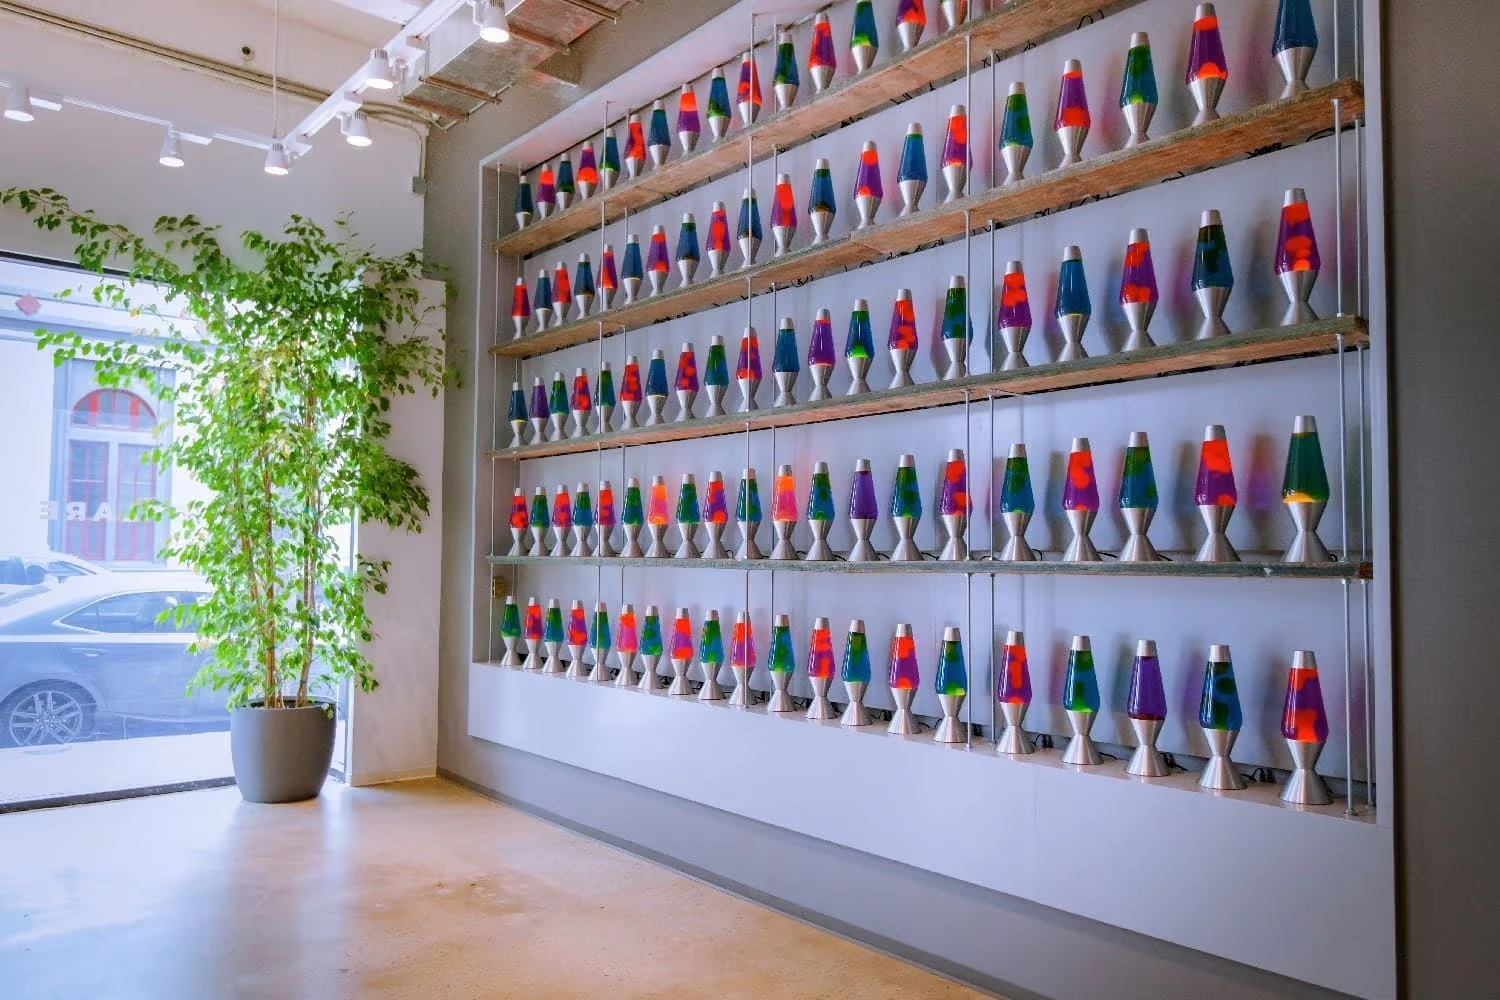
\includegraphics[width=0.85\textwidth]{images/lavaLampCloudFlare}
  \caption{Lávové lampy ako fyzikálny zdroj náhodnosti}
  \label{fig:lava-lamps}
\end{figure}


%-----------------------------------------------------------------------------------------------------------------------------------------------------------

\chapter{Testovanie náhodných čísel}\label{ch:testovanie-nahodnych-cisel}

Ako uvádza Národný inštitút pre štandardy a technológie (NIST) vo svojej publikácii \textit{A Statistical Test Suite for Random and Pseudorandom Number Generators for Cryptographic Applications}~\cite{NIST_SP800-22}, aj malé odchýlky od ideálnej náhodnosti môžu viesť k predvídateľnosti, čo je obzvlášť nebezpečné v kryptografických aplikáciách. Podobne Bastos a kol.~\cite{Bastos2020_ON_PRNG} upozorňujú, že mnohé pseudonáhodné generátory zlyhávajú pri určitých testoch a tým ohrozujú integritu systémov, ktoré na nich závisia.

Nie všetky náhodné čísla sú si teda rovné – a generátory, ktoré sa môžu na prvý pohľad javiť ako náhodné, nemusia byť v skutočnosti náhodné. Preto je nevyhnutné podrobovať ich prísnemu testovaniu a overovaniu prostredníctvom štandardizovaných testovacích balíkov, ako sú napríklad NIST STS, Dieharder alebo TestU01, ktoré umožňujú objektívne posúdiť kvalitu a entropiu generovaných sekvencií.

\section{Teoretické základy náhodnosti a Bellove páry}\label{sec:teoreticke-zaklady-nahodnosti-a-bellove-pary}

Z fyzikálneho hľadiska je náhodnosť úzko spojená s princípmi kvantovej mechaniky. Kým klasická fyzika opisuje svet deterministicky, kvantová mechanika pracuje s pravdepodobnostným charakterom meraní. Jedným z najdôležitejších javov potvrdzujúcich skutočnú kvantovú náhodnosť je \textbf{kvantové prepletenie} (entanglement).

Aby sme mohli kvantitatívne vyjadriť úroveň náhodnosti a prepletenia kvantových stavov, použijeme pojem \textbf{von Neumannova entropia}, tak ako je zadefinovaná v publikácii \textit{Quantum Computation and Quantum Information} od Michaela Nielsena a Isaaca Chuanga~\cite{nielsen_chuang_2010}. Táto veličina predstavuje mieru neurčitosti (alebo informácie), ktorá je obsiahnutá v kvantovom stave. V prípade prepletených systémov vyjadruje stupeň kvantovej korelácie medzi dvoma časticami.

Uvažujme ideálny \textbf{Bellov stav} označovaný ako $\lvert \Phi^+ \rangle$, ktorý je maximálne prepleteným stavom dvoch qubitov:

\begin{equation}
  \lvert \Phi^+ \rangle = \frac{1}{\sqrt{2}}\left(\lvert 00 \rangle + \lvert 11 \rangle\right)
  \label{eq:perfect_bell_pai}
\end{equation}

Tento stav predstavuje ideálnu situáciu, v ktorej majú kombinácie $\lvert 00 \rangle$ a $\lvert 11 \rangle$ rovnakú pravdepodobnosť $50/50$. To znamená, že ak vykonáme meranie na jednom z qubitov, jeho výsledok bude úplne náhodný, avšak výsledky oboch qubitov budú dokonale korelované.

\paragraph{Hustotná matica systému}

Pre daný čistý stav môžeme zostaviť hustotnú maticu celého dvojqubitového systému $\rho_{AB}$:


\begin{equation}
  \rho_{AB} = \lvert \Phi^+ \rangle \langle \Phi^+ \rvert = \frac{1}{2}
  \begin{pmatrix}
    1 & 0 & 0 & 1 \\
    0 & 0 & 0 & 0 \\
    0 & 0 & 0 & 0 \\
    1 & 0 & 0 & 1
  \end{pmatrix}
  \label{eq:bell_pair_matrix}
\end{equation}


Táto matica opisuje celý systém dvoch prepletených qubitov ako jeden celok.

\paragraph{Redukovaná hustotná matica}

Aby sme zistili entropiu jednej časti systému (napríklad qubitu A), musíme „zosledovať“ druhú časť systému, teda vykonať tzv. \textit{čiastočnú stopu} (angl. \textit{partial trace}) nad qubitom B. Tým získame \textbf{redukovanú hustotnú maticu} $\rho_A$:


\begin{equation}
  \rho_A = \mathrm{Tr}_B(\rho_{AB}) = \frac{1}{2}
  \begin{pmatrix}
    1 & 0 \\
    0 & 1
  \end{pmatrix}
  \label{eq:bell_pair_reduced_matrix}
\end{equation}


Takto získaná matica zodpovedá maximálne zmiešanému stavu – čo znamená, že pre jednotlivý qubit neexistuje žiadna informácia o tom, v akom stave sa nachádza. Pravdepodobnosť, že sa qubit nachádza v stave $\lvert 0 \rangle$ alebo $\lvert 1 \rangle$, je presne rovnaká.

\paragraph{Výpočet von Neumannovej entropie}

Von Neumannova entropia sa pre danú hustotnú maticu $\rho$ vypočíta podľa vzorca:

\begin{equation}
  S(\rho) = -\mathrm{Tr}(\rho \log_2 \rho) = - \sum_i \lambda_i \log_2 \lambda_i,
  \label{eq:neaumab_entropy}
\end{equation}

kde $\lambda_i$ sú vlastné hodnoty hustotnej matice.

V našom prípade má $\rho_A$ dve rovnaké vlastné hodnoty $\lambda_1 = \lambda_2 = \frac{1}{2}$. Preto dostávame:

\begin{equation}
  S(\rho_A) = - \left( \frac{1}{2} \log_2 \frac{1}{2} + \frac{1}{2} \log_2 \frac{1}{2} \right) = 1
  \label{eq:neaumab_entropy_modified_to_fit}
\end{equation}

\paragraph{Interpretácia výsledku}

Získaný výsledok $S(\rho_A) = 1$ znamená, že entropia – a teda aj miera náhodnosti či nepredvídateľnosti stavu – je \textbf{maximálna}.
Tento stav predstavuje teoretický limit pre dvojicu kvantovo prepletených častíc. Každé meranie jedného z qubitov vedie k úplne náhodnému výsledku, pričom systém ako celok ostáva dokonale korelovaný.

Preto možno konštatovať, že Bellov pár typu $\lvert \Phi^+ \rangle$ je \textbf{maximálne prepletený a predstavuje ideálny zdroj skutočnej kvantovej náhodnosti}, pričom teoretická hodnota von Neumannovej entropie pre jeden qubit v takomto stave je presne \textbf{1 bit}.

\section{Metódy testovania náhodnosti}\label{sec:statisticke-testy-nahodnosti}

Na praktické overenie kvality generovaných čísel sa využívajú rôzne štatistické testovacie metódy.
Tieto testy analyzujú vlastnosti sekvencií bitov alebo čísel s cieľom zistiť, či sa správanie výstupu zhoduje s očakávaným správaním skutočne náhodného zdroja.

Pri hodnotení kvality náhodnosti sa sledujú najmä tieto vlastnosti:
rovnomernosť rozdelenia bitov, absencia deterministickej štruktúry, stabilita vlastností sekvencie v čase a nepredikovateľnosť budúcich hodnôt.

V rámci tejto práce boli použité viaceré typy testov, ktoré možno rozdeliť do troch hlavných skupín:
základné štatistické testy inšpirované metodikou NIST, testy založené na predikcii nasledujúceho bitu a analýzy stability bitového toku.

\subsection{NIST Statistical Test Suite}\label{subsec:nist-statistical-test-suite}


\textbf{NIST STS} (National Institute of Standards and Technology Statistical Test Suite)~\cite{NIST_SP800-22} patrí medzi najrozšírenejšie nástroje používané pri testovaní kryptografických generátorov náhodných čísel.
Obsahuje viac než 15 rôznych testov, ktoré analyzujú rôzne vlastnosti bitových sekvencií.

V rámci tejto práce boli implementované vybrané testy inšpirované touto metodikou, ktoré analyzujú základné štatistické vlastnosti bitového toku:

\begin{itemize}
  \item \textbf{Test vyváženosti bitov} – skúma rovnomernosť výskytu núl a jednotiek v sekvencii.
  Ide o jeden zo základných testov náhodnosti, ktorý overuje, či sa počet bitov $0$ a $1$ približne rovná.

  \item \textbf{Test behov bitov} – analyzuje počet a dĺžku po sebe idúcich rovnakých bitov.
  Výrazné odchýlky od očakávaného počtu behov môžu naznačovať prítomnosť deterministickej štruktúry v sekvencii.

  \item \textbf{Test kumulatívneho súčtu} – sleduje vývoj kumulatívneho súčtu bitov interpretovaných ako náhodná prechádzka.
  Výrazný drift kumulatívneho súčtu môže indikovať systematickú nerovnováhu v bitovom toku.
\end{itemize}

Sekvencia je v rámci týchto testov považovaná za náhodnú, ak vypočítaná p-hodnota testu presiahne zvolenú hranicu významnosti.

\subsection{Analýza stability bitového toku}

Okrem základných štatistických testov bola v práci vykonaná aj \textbf{analýza rozdelenia bitového toku}.
Táto analýza skúma, či sa štatistické vlastnosti generovaného bitového toku nemenia v priebehu generovania.

Bitový tok je rozdelený na viacero segmentov a pre každý segment sa samostatne vyhodnocujú:
\begin{itemize}
  \item podiel núl ($p_{\text{nuly}}$),
  \item podiel jednotiek ($p_{\text{jednotky}}$),
  \item odchýlka od ideálneho pomeru $0{,}5$.
\end{itemize}

Cieľom tejto analýzy je odhaliť prípadné lokálne skreslenia alebo nestabilitu generátora v priebehu generovania.

Súčasťou experimentov bola aj analýza rozdelenia bitového toku po aplikovaní extrakcie entropie pomocou kryptografickej hašovacej funkcie MD5.
Táto transformácia sa používa na rozptýlenie lokálnych štruktúr a odstránenie prípadných systematických odchýlok vo vstupnom signáli.

\section{Kryptografická odolnosť a \textit{next-bit test}}\label{sec:kryptograficka-bezpecnost-a-textit{next-bit-test}}

V kontexte kryptografie nestačí, aby boli náhodné čísla iba štatisticky rovnomerné – musia byť aj \textbf{nepredvídateľné}.
Základným konceptom, ktorý tento princíp formalizuje, je tzv. \textbf{next-bit test}.

Podľa definície Blum a Micali (1984) je generátor kryptograficky bezpečný, ak žiadny polynomiálny algoritmus nedokáže s pravdepodobnosťou väčšou ako 0,5 predpovedať nasledujúci bit sekvencie, aj keď pozná všetky predchádzajúce bity~\cite{BlumMicali1984}.

V tejto práci bola táto myšlienka overovaná pomocou dvoch typov prediktívnych testov.

Prvým bol \textbf{test predikcie nasledujúceho bitu}, ktorý využíva model strojového učenia na predikciu ďalšieho bitu na základe predchádzajúcich hodnôt.
Výsledky sú vyhodnocované pomocou metrík presnosť predikcie, vyvážená presnosť, schopnosť rozlišovania tried a logaritmická strata predikcie.

Druhým použitým testom bol \textbf{Markovov test}, ktorý vychádza z Markovovho modelu prvého rádu.
Tento test skúma, či pravdepodobnosť nasledujúceho bitu závisí od bezprostredne predchádzajúceho bitu.

Ak žiadny z týchto prediktívnych prístupov nedokáže predpovedať nasledujúci bit lepšie než náhodným hádaním, možno usudzovať, že sekvencia neobsahuje jednoducho využiteľnú deterministickú štruktúru.
